\section{Theoretical Model}
  \label{sec:simultons_theory}

    We start with a quantised three-level atom as illustrated in figure
    \ref{fig:vee_schematic}. The probe beam couples the ground state $\Ket{0}$
    to an excited state $\Ket{1}$ while an orthogonal coupling beam couples
    $\Ket{0}$ to an adjacent excited state $\Ket{2}$. The transition $\Ket{1}$
    to $\Ket{2}$ is dipole-forbidden, completing the definition of the V-type
    atom. With this simplified model of the atomic system, we are neglecting the
    hyperfine structure of the $5^2\mathrm{S}_{\nicefrac{1}{2}}$,
    $5^2\mathrm{P}_{\nicefrac{1}{2}}$ and $5^2\mathrm{P}_{\nicefrac{3}{2}}$
    states. We will discuss this approximation further in section
    \ref{sec:simultons_long}.

    The total electric field vector for the two laser beams is described by
    \begin{equation}
      \mathbf{E}(z,t) = \left[ \tfrac{1}{2} \mathbf{\hat{x}}_p 
        \mathcal{E}_p(z,t) \ee^{\ii(k_p z - \omega_p t)} + 
        \tfrac{1}{2} \mathbf{\hat{x}}_c \mathcal{E}_c(z,t) \ee^{\ii(k_c z -
        \omega_c t)} + \cc \right]
      \label{eqn:env_carrier}
    \end{equation}
    where $\mathbf{\hat{x}}_p$ and $\mathbf{\hat{x}}_c$ are orthogonal
    polarisation of the vectors of the fields and the envelopes $\mathcal{E}_p$
    and $\mathcal{E}_c$ are in general complex functions. We define
    corresponding Rabi frequencies $\Omega_p = d_{01}\mathcal{E}_p/\hbar$ and
    $\Omega_c = d_{02}\mathcal{E}_c/\hbar$ where $d_{0j}$ is the dipole moment
    between levels $\Ket{0}$ and $\Ket{j}$, which we take parallel to its
    respective field polarisation.

    The Hamiltonian for the V-type three-level atom interacting with these two 
    classical fields is
    \begin{equation}
      \mathcal{H}_\mathrm{V} = -\hbar (\Delta_p \sigma_{11} + \Delta_c 
      \sigma_{22}) -\frac{\hbar}{2} 
      \left[ (\Omega_p \sigma_{10} + \Omega_c \sigma_{20} )
      + \hc \right]
      \label{eqn:vee_hamiltonian}
    \end{equation}
    within the dipole approximation and in the frame rotating with the
    frequencies of the optical fields. Here again $\sigma_{ij} := \Ket{i}\Bra{j}$ is
    the transition operator. Along with accounting for off-resonant fields, the
    inclusion of detunings $\Delta_p$ and $\Delta_c$ allows us to consider
    Doppler broadening via an atom distribution $P(\Delta)$ as described in
    chapter \ref{chp:propagation}.

    Armed with this Hamiltonian we can apply the semiclassical Maxwell-Bloch
    propagation models described in chapter \ref{chp:propagation} to solve for
    the electric fields $\mathcal{E}_{p,c}$ and atomic density operator $\rho$
    over $z$ and $t$ as the fields move through the medium.

    The temporal profile of the \textsc{cw} probe and Gaussian pulsed
    coupling input at the front of the medium ($z\!=\!0$) constitute the
    necessary boundary condition on the fields.

    Switching on the \textsc{cw} probe field instantaneously from zero to
    $\Omega_{p0}$ would introduce a discontinuity and thus spurious ringing due
    to the Gibbs phenomenon.\cite{Hewitt1979}. We thus construct a switch-on
    function which ramps up smoothly. We take a real-valued $\Omega_{p}$
    function
    \begin{equation}
      \Omega_p(z\!=\!0, t) = 
      \begin{cases}
        \Omega_{p0} \exp \left[ -4 \log 2 \left( \frac{t - t_0}{t_w}
        \right)^2 \right] & t < t_0\\
        \Omega_{p0} & t \ge t_0
      \end{cases}
    \end{equation}
    where $t_0$ is the point at which the function reaches its peak
    $\Omega_{p0}$. The duration of the ramp-on is governed by $t_w$, which is
    the full width at half maximum (\textsc{fwhm}) of a Gaussian. We also
    require an initial condition for the atomic states, where it is reasonable
    to assume negligible population in either of the excited states.

    The interaction Hamiltonian allows us to follow coherent evolution of pure
    atomic states. To our analysis we will also include the interaction of atoms
    with  the environment via spontaneous decay of excited states. We'll still
    be considering coupling pulses much shorter than the decay time associated
    with  this decay as discussed in chapter \ref{chp:nonlinear}.

    The spontaneous decay effect is included in the model via collapse operators
    $C_j$ in the Lindblad equation (\ref{eqn:lindblad}) describing time evolution
    of the atomic states. For the V configuration atom we have $C_{j}  =
    \sqrt{\Gamma_{0j}}\sigma_{0j}$ for $j \in \{1, 2\}$ representing spontaneous
    decay of the excited states, where $\Gamma_{0j}$ are the decay rates.

  \subsection{Simulation Results}

    With this theoretical model, we are now in a position to set up and run
    numerical simulations of the physical system using the Maxwell-Bloch
    propagation algorithm described in Appendix \ref{apx:mb_eqns}.

    We present results of an example simulation in figures
    \ref{fig:sim_0703_temp_210C_build0_fields},
    \ref{fig:sim_0703_temp_210C_build0_pop} and
    \ref{fig:sim_0703_temp_210C_build0_coh}. In this example we take a rubidium
    cell of length $L = $ \unit[$2$]{$\mu$m} at a temperature $T =
    \unit[230]{\textrm{\textdegree C}}$, which translates to absorption
    coefficients of $Ng_{01} = \unit[2\pi~66.7]{\Gamma/L}$ and $Ng_{02} =
    \unit[2\pi~128]{\Gamma/L}$ (see chapter \ref{chp:propagation} for a
    description of the absorption coefficients). Given the decay time $\tau =
    1/\Gamma_{01}$, the input ($z\!=\!0$) coupling pulse has a \textsc{fwhm} of
    $t_w = $ \unit[$0.029$]{$\tau$}, (equivalent to \unit[$0.80$]{ns}), a peak
    of $\Omega_c = \unit[2\pi~130]{\Gamma}$ (\unit[$2\pi~748$]{MHz}) and is
    centred at $t\!=\!0$. The \textsc{cw} probe is ramped up to $\Omega_p = $
    \unit[$2\pi~15$]{$\Gamma$} (\unit[$2\pi~86$]{MHz}) long enough before the
    pulse (at $t = $ \unit[$-1.5$]{$\tau$}) for the system to reach a steady
    state.

    \begin{figure}%[h]
      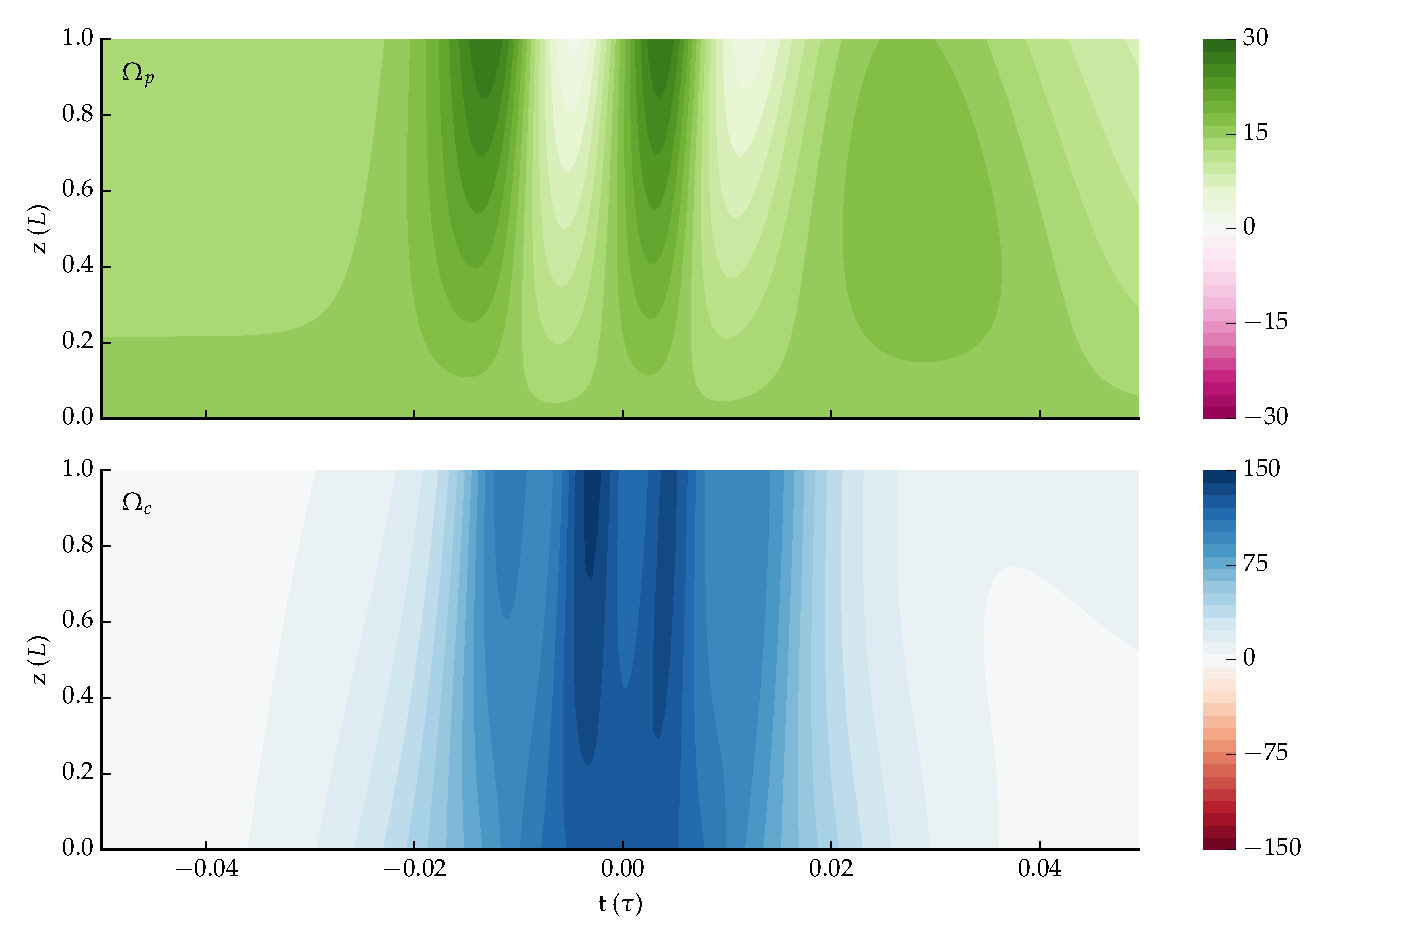
\includegraphics[width=\linewidth]
        {figs/06_simultons/mb_vee2g_build0_15c_130p_0330t_230C_sb50_120vel000_00_002um_fig2.pdf}
      \caption{
      Real parts of the complex Rabi frequencies $\Omega_{p}$ (top) and
      $\Omega_{c}$ (bottom) in the simulated pulse/\textsc{cw} scheme. The
      coupling pulse has width $t_w = $ \unit[$0.029$]{$\tau$} and peak
      $\Omega_c$ of \unit[$2\pi~130$]{$\Gamma$}. The absorption coefficients are
      $Ng_{01} = \unit[2\pi~66.7]{\Gamma/L}$ and $Ng_{02} =
      \unit[2\pi~128]{\Gamma/L}$.
      }
      \label{fig:sim_0703_temp_210C_build0_fields}
    \end{figure}

    In figure \ref{fig:sim_0703_temp_210C_build0_fields} we look at the
    evolution of the fields, as described by the real part of the complex Rabi
    frequencies $\Omega_p$ and $\Omega_c$, in the time window around the pulse.
    The contoured colour maps correspond to the real parts of $\Omega_p$ and
    $\Omega_c$ according to the colour scale on the right, with local time $t'$
    on the $x$-axis (these results are displayed in the co-moving reference
    frame) and the distance $z$ that the fields travel through the medium on the
    $y$-axis. The input boundary conditions are thus represented by a horizontal
    slice at at $z\!=\!0$.

    We see that the coupling pulse (bottom) is not attenuated over this
    distance, but in fact is shaped and is indeed amplified and split around the
    centre ($t=0$). A long-time tail emerges towards the end of the medium
    ($z\!=\!L$).

    \begin{figure}%[h]
      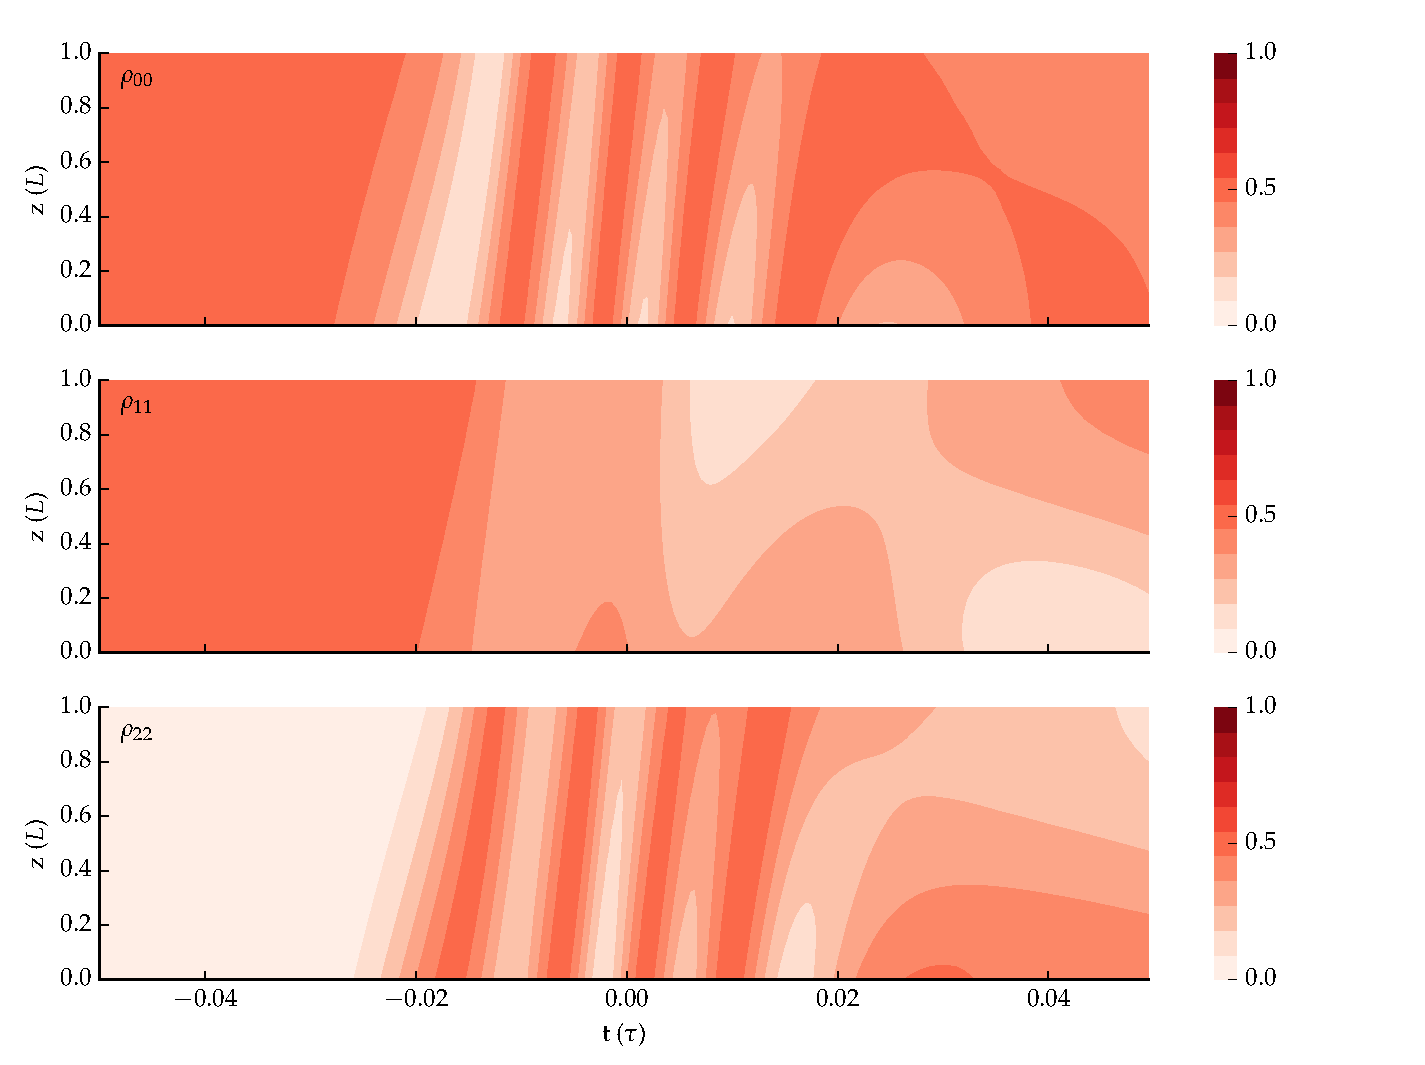
\includegraphics[width=\linewidth]{figs/06_simultons/mb_vee2g_build0_15c_130p_0330t_230C_sb50_120vel000_00_002um_fig3.pdf}
      \caption{
      Populations of the ground state $\rho_{00}$ (top) and excited states
      $\rho_{11}$ (middle) and  $\rho_{22}$ (bottom) over $z$ and $t'$  in the
      simulated pulse/\textsc{cw} scheme, with parameters as those in figure
      \ref{fig:sim_0703_temp_210C_build0_fields}.
      }
      \label{fig:sim_0703_temp_210C_build0_pop}
    \end{figure}

    Before the pulse, the \textsc{cw} probe field (top) is attenuated as it
    progresses through the medium, as we would expect from the usual Beer law of
    absorption. This behaviour is abruptly disturbed by the coupling pulse,
    however. In response to the arriving pulse, the probe field is first
    amplified over a period of about \unit[$0.01$]{$\tau$} and then strongly
    attenuated, and this process repeats twice over the duration of the pulse.
    After the pulse the field returns to its initial state.

    \begin{figure}%[h]
      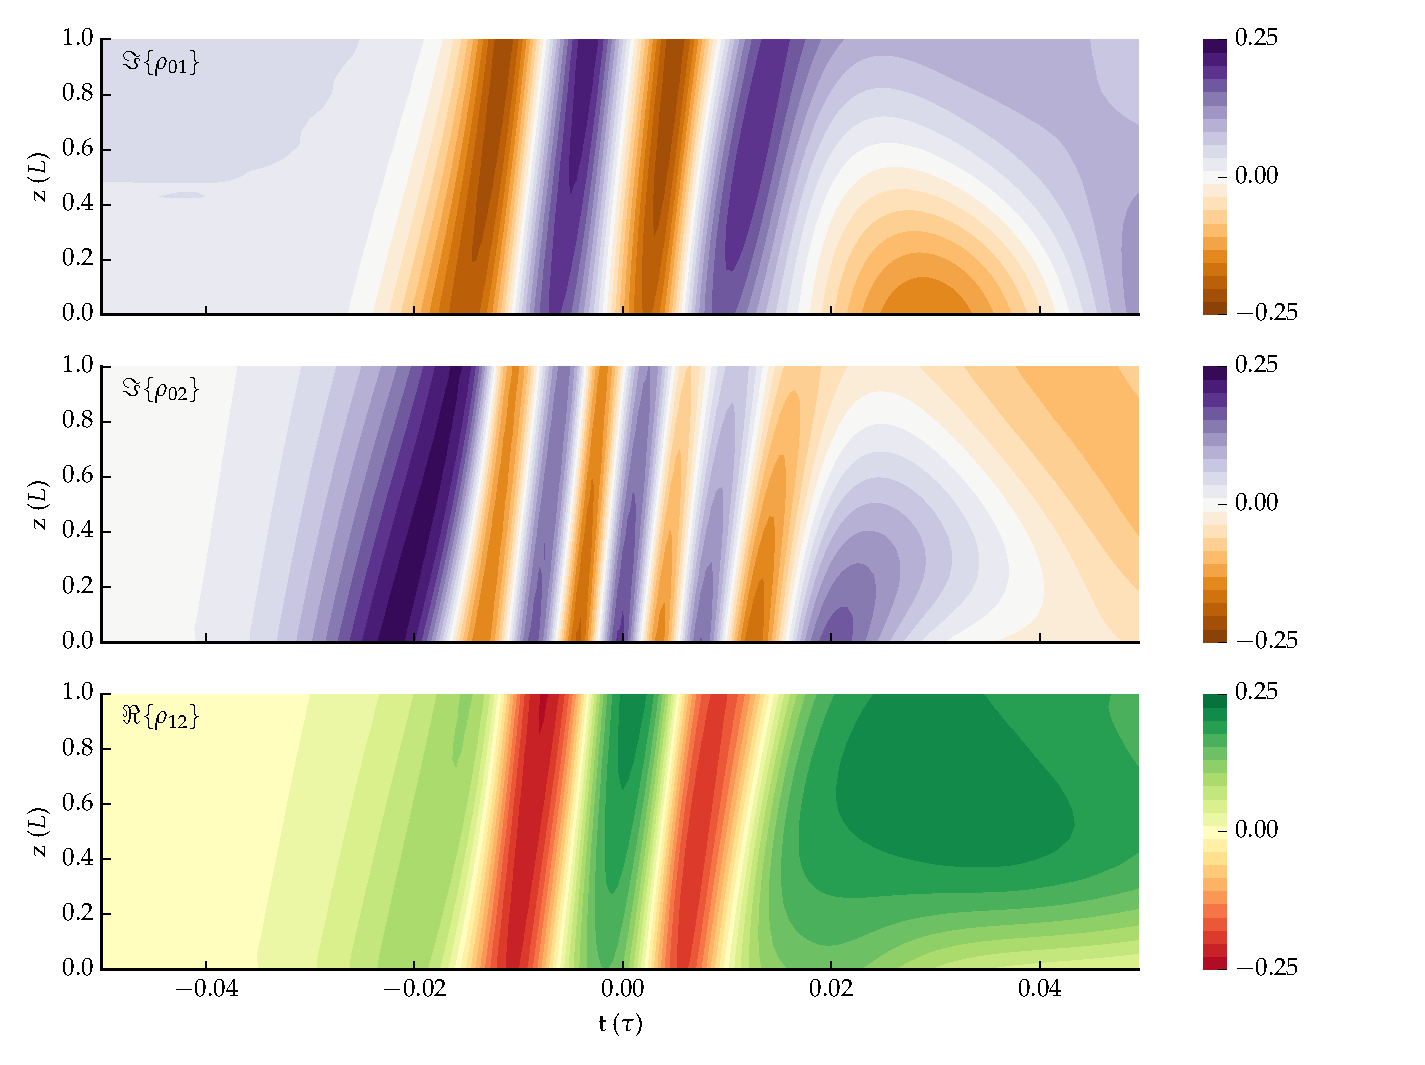
\includegraphics[width=\linewidth]
        {figs/06_simultons/mb_vee2g_build0_15c_130p_0330t_230C_sb50_120vel000_00_002um_fig4.pdf}
      \caption{
      Selected coherences of the atomic density matrix. The imaginary parts of
      $\rho_{01}$ (top) and $\rho_{02}$ (middle) and the real part of
      $\rho_{12}$ (bottom) over $z$ and $t'$ in the simulated pulse/\textsc{cw}
      scheme, with parameters as those in figure
      \ref{fig:sim_0703_temp_210C_build0_fields}.
      }
      \label{fig:sim_0703_temp_210C_build0_coh}
    \end{figure}

    In figure \ref{fig:sim_0703_temp_210C_build0_pop} we look at the evolution
    of the atomic populations of the states $\Ket{0}$, $\Ket{1}$ and $\Ket{2}$
    during the same window as figure \ref{fig:sim_0703_temp_210C_build0_fields},
    with local time $t'$ on the $x$-axis and the distance $z$ that the fields
    travel through the medium on the $y$-axis. These diagonal elements of the
    density matrix are real and must sum to unity as expressed in equation
    (\ref{eqn:density_matrix_trace}), and so the colour scale is from zero to
    one on each plot.

    We see that the population is initially divided evenly between $\rho_{00}$
    (top) and $\rho_{11}$ (middle), with no population in the $\Ket{2}$ state,
    as expected since initially the medium is in the steady state driven on
    resonance by the \textsc{cw} probe field. During the pulse population is
    driven between $\rho_{00}$ and $\rho_{22}$ (bottom). The population in
    $\rho_{11}$ is reduced during the pulse. The small positive slope of these
    features on each of the colour maps shows the pulse arriving later in time
    relative to the  speed-of-light frame as the fields move through the medium.
    This corresponds to a slow-light refractive index (see chapter
    \ref{chp:polaritons}).

    In figure \ref{fig:sim_0703_temp_210C_build0_coh} we look at the evolution
    of the off-diagonal density matrix elements during the same window. Some
    interesting behaviour of the system is demonstrated here. The top two
    subplots with orange-to-purple colour maps, show imaginary parts of
    coherences $\rho_{01}$ and $\rho_{02}$ between the ground state and the two
    excited states. The bottom subplot, with red-to-green colour map, shows the
    real part of the $\rho_{12}$ coherence between the two excited states,
    corresponding to phase coherence between these states.

    Firstly, we note that the $\Im\{\rho_{02}\}$ coherence (middle) makes around
    four complete oscillations during the pulse, corresponding to the strong
    driving field. Secondly, $\Im\{\rho_{01}\}$ (top) makes around two
    oscillations but out-of-phase with $\Im\{\rho_{02}\}$ such that it is first
    driven negative. Finally, $\Re\{\rho_{12}\}$ (bottom) is nonzero such that
    there is a real coherence between the two excited states despite them not
    being coupled directly. This oscillates on the same timescale as
    $\Im\{\rho_{01}\}$.

    The fact that we see such strong early amplification of the probe field in
    figure \ref{fig:sim_0703_temp_210C_build0_fields} suggests that this model
    includes the cause of the pulse steepening observed in experiment, however
    there are some important physical mechanisms we should include in order to
    simulate the system accurately, and we will consider these now.

  \subsection{Inhomogeneous Broadening}

    As the experiments described in section \ref{sec:simultons_experiment}
    involved thermal atoms, in order to compare these results with our numerical
    simulations we need to include some important averaging and dephasing
    effects due to the motion of the atoms.

    Due to the Doppler effect the motion of the atoms along
    the $z$-axis results in a \textsc{1d} Maxwell-Boltzmann probability
    distribution function over detuning\cite{foot2005atomic, Gea-Banacloche1995}
    \begin{equation}\label{eqn:max_boltz}
      f(\Delta) = \tfrac{1}{u \sqrt{\pi}} \ee^{-(\Delta/u)^2}
    \end{equation}
    where the thermal width $u = k v_w$. Here $k$ is again the wavenumber of the quasi-monochromatic field and $v_w = 2 k_B T/m$ is the most probable speed of the Maxwell-Boltzmann distribution for a temperature $T$ and atomic mass $m$.
    \cite{schroeder2000introduction}

    To include this effect in the field propagation equations, as described in chapter \ref{chp:propagation}, we replace the atomic coherence factor by an
    integral over the convolution of $P(\Delta)$ with the atomic coherence now a function of detuning, so that
    \begin{subequations}\label{eqn:mwe_svea_doppler}
    \begin{align}
      \frac{\partial \Omega_p}{\partial \zeta}(\zeta, \tau) = \ii N g_{01} 
      \int_{-\infty}^{\infty} \rho_{01}(\zeta, \tau, \Delta) f(\Delta) \dd 
      \Delta, \\
      \frac{\partial \Omega_c}{\partial \zeta}(\zeta, \tau) = \ii N g_{02} 
      \int_{-\infty}^{\infty} \rho_{02}(\zeta, \tau, \Delta) f(\Delta) \dd
      \Delta.
    \end{align}
    \end{subequations}

  \subsection{Collision Dephasing}

    We also consider that a thermal cloud of atoms is randomly distributed and
    that moving atoms will collide with one another. Transient dipole-dipole
    interactions between colliding atoms leads to a dephasing of dipoles and an
    additional broadening. We account for this effect by
    defining a \textit {self-broadening} coefficient $\beta$ and a parameter
    known as the Weisskopf radius\cite{Lewis1980}
    \begin{equation}\label{eqn:weisskopf}
      r_W = \sqrt{\frac{\beta}{2\pi \bar{v}}}
    \end{equation}
    where
    \begin{equation}\label{eqn:mean_vel}
    \bar{v} = 2 \sqrt{\frac{2}{\pi}} v_w
    \end{equation}
    is the expected relative speed of a pair of atoms. We may make a
    \textit{binary approximation}, considering that all collisions involve only
    two atoms, on the condition that\cite{thorne1999spectrophysics}
    \begin{equation}\label{eqn:weisskopf_cond}
      \tfrac{4\pi}{3}Nr_W^3 < 1
    \end{equation}
    which means that in a sphere around any given atom with a radius $r_W$, we
    will expect to find at most one other atom. This dephasing effect is then included via additional off-diagonal decay terms
    \begin{equation}\label{eqn:collision_broad}
      \Gamma_{col,j} = N \beta_j = 
        N \frac{d^2}{3 \hbar \varepsilon_0}\sqrt{\frac{2J'+1}{2J+1}}
    \end{equation}      
    where $2J + 1$ and $2J' + 1$ are the fine structure multiplicities of the
    ground and excited states.\cite{Weller2011, Lewis1980} Collision broadening
    thus has the effect of increasing uncertainty in the off-diagonal terms.

    For rubidium thermal vapour we have $\beta_{\textsc{d1}} = $
    \unit[$2\pi~0.73$]{MHz $\mu$m$^3$}  and $\beta_{\textsc{d2}} = $
    \unit[$2\pi~1.03$]{MHz $\mu$m$^3$} for the \textsc{d} line
    transitions.\cite{Weller2011} The binary approximation then breaks down only
    at a density of $N \approx \unit[10^{17}]{cm^{-3}}$ corresponding to a
    temperature of $T = \unit[360]{\textrm{\textdegree C}}$, and so is a good
    approximation across the temperature range of the experiment.

    \begin{figure}[h]
      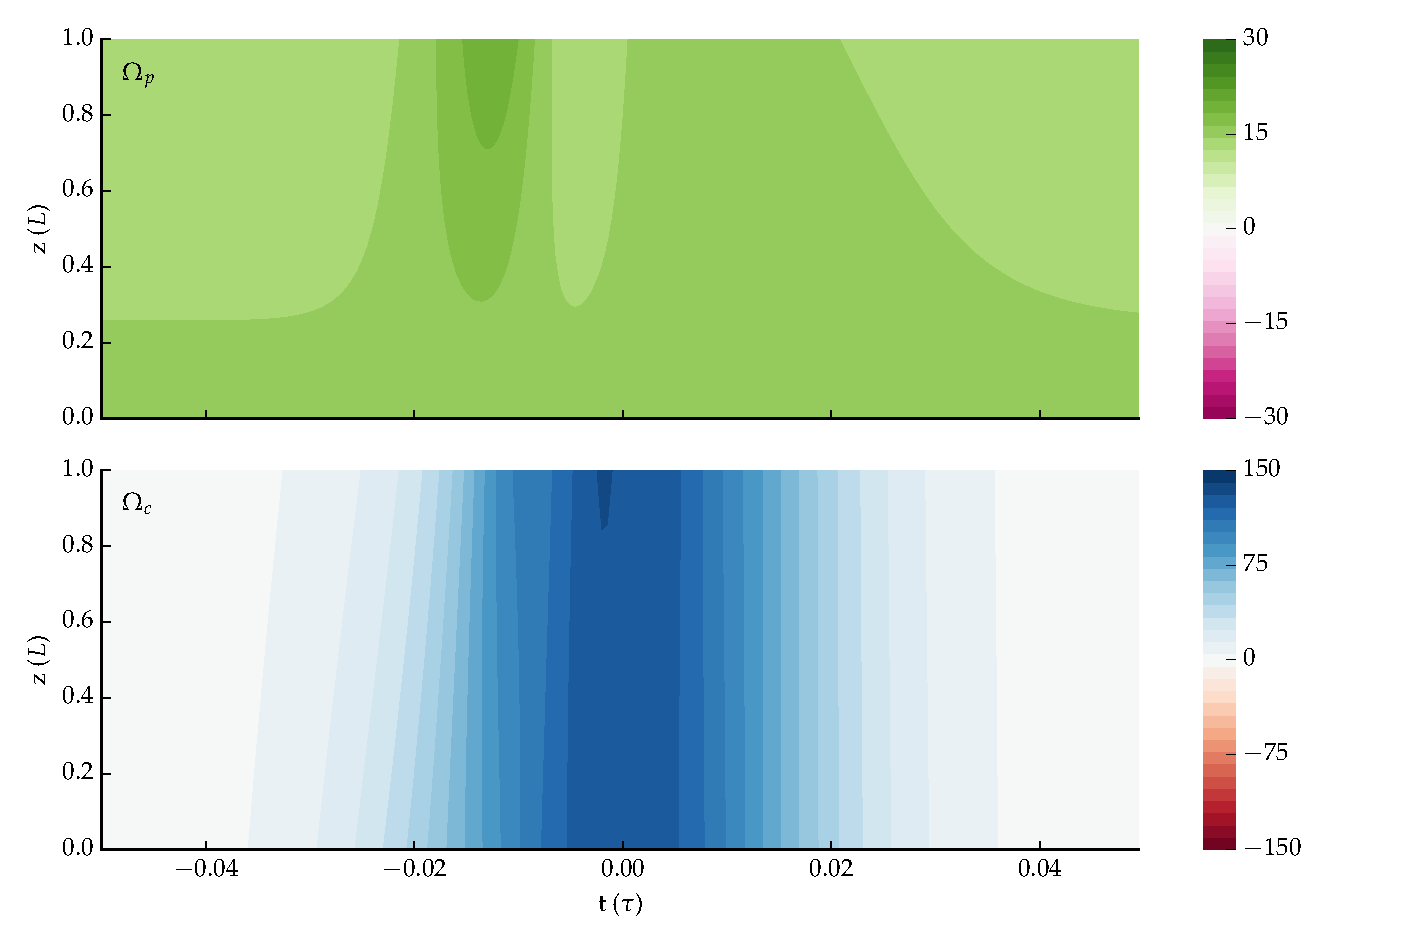
\includegraphics[width=\linewidth]{figs/06_simultons/mb_vee2g_build1_15c_130p_0330t_230C_sb50_120vel000_00_002um_fig2.pdf}
      \caption{Real parts of the complex Rabi frequencies $\Omega_{p}$ (top) and 
      $\Omega_{c}$ (bottom) in the simulated pulse/\textsc{cw} scheme for the parameter set in figure \ref{fig:sim_0703_temp_210C_build0_fields}, with the inclusion of motional effects of Doppler and collision broadening.}
      \label{fig:sim_0703_temp_210C_build2_fields}
    \end{figure}

    In figure \ref{fig:sim_0703_temp_210C_build2_fields} we again show the
    evolution of the real part of the complex Rabi frequencies $\Omega_p$ and
    $\Omega_c$ for the model in figure
    \ref{fig:sim_0703_temp_210C_build0_fields}, but this time with the inclusion
    of the motional effects described. 

    We no longer see the level of amplification and splitting on the coupling
    pulse that we saw in figure \ref{fig:sim_0703_temp_210C_build0_fields}, with
    the pulse maintaining its profile through the medium. The strong
    amplification and attenuation on the \textsc{cw} probe field has also been
    damped significantly, particularly on the second oscillation. The periods of
    attenuation return the field Rabi frequency to the level observed without
    the pulse over this distance.

  \subsection{Hyperfine Pumping}

    The final physical mechanism we include in our model is that of
    optical \textit{hyperfine pumping}, which will affect the propagation of
    both fields.\cite{Razdan1999,Im2001,Nakayama1985}

    A rubidium atom with nuclear spin $I$ has two angular momentum values for
    the ground state: $F\!=\!I\!\pm\!\nicefrac{1}{2}$. The hyperfine splitting
    of this ground state is on the order of \unit{GHz}, whereas the splitting on
    the $5$P excited states is on the order of \unit{MHz}, as
    shown in figure \ref{fig:rb85_levels}.

    If the monochromatic field is tuned to the transition from the lower ground
    state to the excited state manifold, the higher ground state is far from
    resonance and so does not couple significantly. The mechanism of decay via
    spontaneous emission to the higher ground state will then remove atoms from
    the probe and coupling system.\cite{Smith2004}

    Atoms that have decayed to the lower ground state are \textit{dark} to the
    optical fields until they are transferred via collision into the higher
    ground state. The transit time of atoms in the beam is shorter than the
    timescale of this transfer by collision so the dark ground state is a sink
    for atomic population, reducing the effective number density and thus
    absorption of the fields.\cite{Sherlock2009}

    To account for hyperfine pumping, we will add a fourth level as a sink to
    the three-level system and adjust our initial condition to evenly populate
    the two ground states. The decay rates $\Gamma_{01}$ and $\Gamma_{02}$ to
    the ground state are then split by branching ratios
    \begin{equation}\label{eqn:hf_branching}
      B_{F \rightarrow J'} = \frac{\sum_{F'} S_{F \rightarrow F'}}{2J' + 1}
    \end{equation}
    where $J, F$ are the orbital and hyperfine angular momentum numbers for the ground state and $J', F'$ are those of the excited state, and the hyperfine strength factors $S_{F \rightarrow F'}$ are given
    by\cite{Steck2001}
    \begin{equation}\label{eqn:strength_factor}
      S_{F \rightarrow F'} = (2F' + 1)(2J + 1)
        \begin{Bmatrix}
        J & J' & 1 \\
        F' & F & I
        \end{Bmatrix}^2.
    \end{equation}

    \begin{figure}[]
      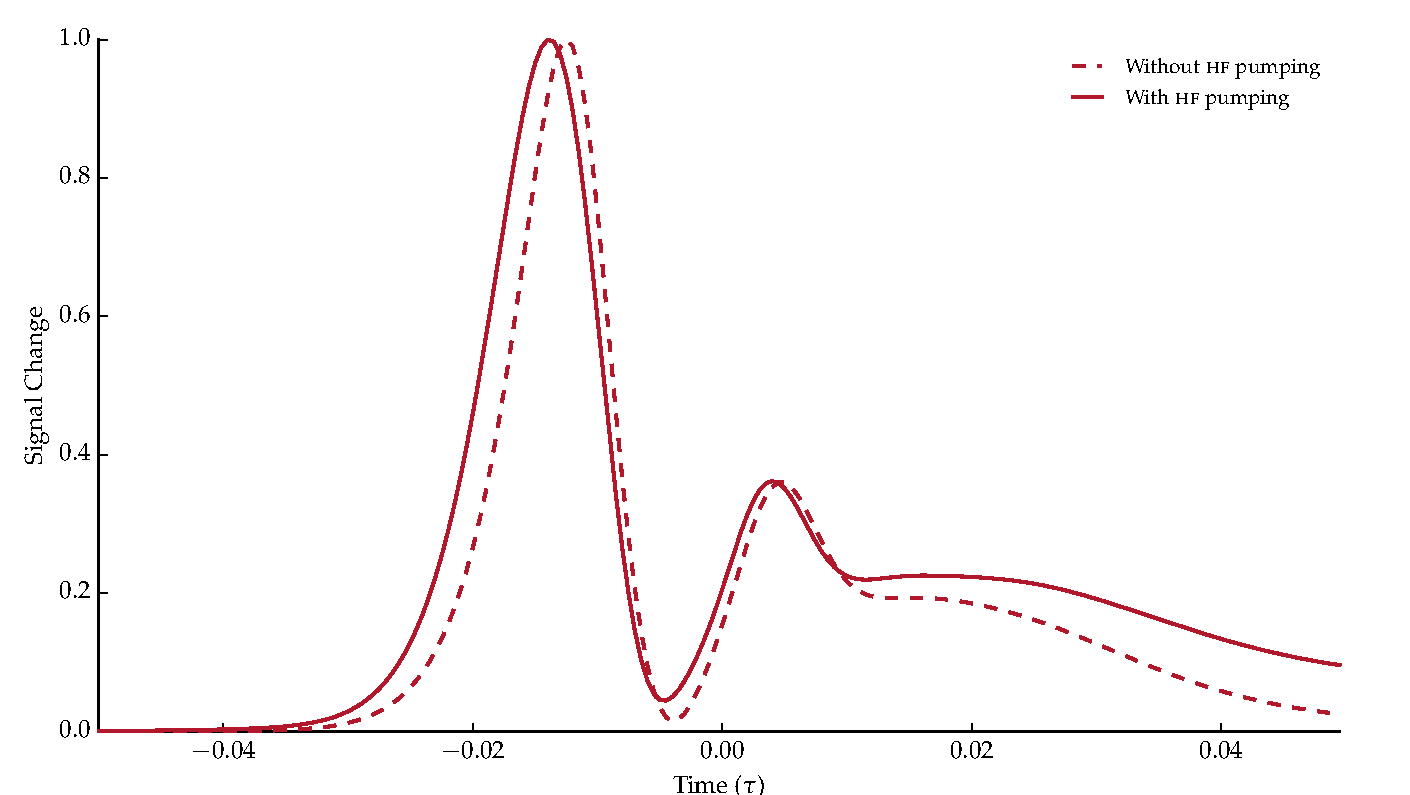
\includegraphics[width=\linewidth]{figs/06_simultons/mb_vee2g_exp_build_plot_1_2_fig1.pdf}
      \caption{
      Simulated transmission intensity at the end of the medium,
      $z=\unit[1]{\textit{L}}$ as the probe responds to the input coupling
      pulse, without hyperfine pumping (red dashed) and with (solid).
      }
      \label{fig:hf_pumping} 
    \end{figure}

    In figure \ref{fig:hf_pumping} we compare results from models with and
    without the addition of hyperfine pumping to a sink state, for the
    transmission observed at the end of the medium, $z=\unit[1]{\textit{L}}$.
    With the inclusion of pumping, we observe that during the simulation the
    absorptive power of the medium decreases as population is trapped in the
    off-resonant dark ground state. This results in an increase in the baseline
    transmitted signal after the pulse with respect to that beforehand. The peak
    with the inclusion of \textsc{hf} pumping is slightly earlier, as the 
    slow-light effect of the medium is reduced with the depopulation of the
    resonantstates.
